\bluepage{Příprava programů a shaderů pro GPU}

\begin{frame}
\frametitle{Dva druhy programovacích jazyků}
   \begin{itemize}
    \item OpenGL standard popisuje i jazyk GLSL
    \item Jazyk GLSL popisuje programy, které běží na GPU
    \item Programátor 3D grafiky píše aplikaci vždy ve 2 jazycích
  \end{itemize}
  \begin{figure}[h]
    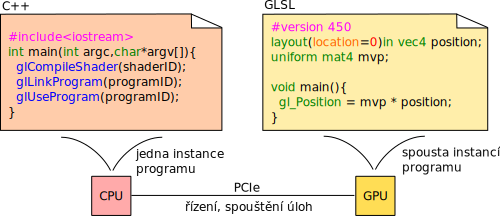
\includegraphics[width=10cm,keepaspectratio]{pics/cpp_and_glsl.pdf}
  \end{figure}
\end{frame}

\begin{frame}
\frametitle{Programy a Shadery}
  \begin{itemize}
  \item Program, který běží na GPU se v OpenGL označuje jako Shader Program
  \item Shader Program je složen z několika částí (stages), které se nazývají Shader
  \item Existuje 6 typů shaderů: \textbf{vertex}, \textbf{fragment}, geometry, tesselation control, tesselation evaluation a compute shader.
  \item Program nemusí obsahovat všechny typy shaderů.
  \item Jednotlivé shadery lze sdílet mezi vícero programy.
  \item Shadery se kompilují (za běhu aplikace)
  \item Programy se linkují (za běhu aplikace)
  \end{itemize}
\end{frame}

\begin{frame}
\frametitle{Kombinace shaderů v programu}
  Validní a často používané kombinace shaderů:
  \begin{figure}[h]
    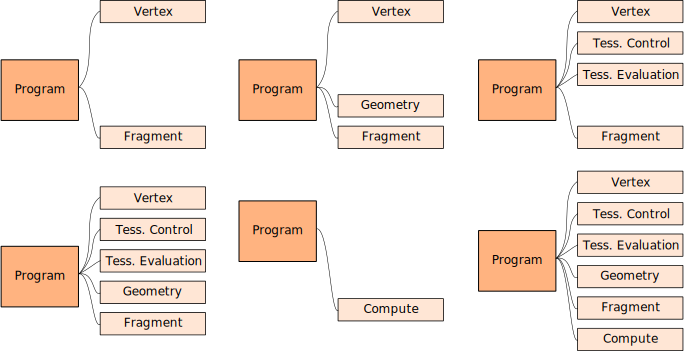
\includegraphics[width=10cm,keepaspectratio]{pics/shader_combination.pdf}
  \end{figure}
\end{frame}

\begin{frame}[fragile]
\frametitle{Kompilace shaderů}
    {\scriptsize
    \begin{minted}[frame=lines]{c++}
template<typename...ARGS>
GLuint compileShader(GLenum type,ARGS... sources){
  std::vector<std::string>str = {std::string(sources)...};
  std::vector<const GLchar*>ptr;
  for(auto x:str)ptr.push_back(x.c_str());

  //reserve shader id
  GLuint id = glCreateShader(type);

  //set shader sources
  glShaderSource(id,(GLsizei)ptr.size(),ptr.data(),nullptr);

  //compile shader
  glCompileShader(id);

  //get compilation log
  GLint bufferLen;
  glGetShaderiv(id,GL_INFO_LOG_LENGTH,&bufferLen);
  if(bufferLen>0){
    char*buffer = new char[bufferLen];
    glGetShaderInfoLog(id,bufferLen,nullptr,buffer);
    std::cerr<<buffer<<std::endl;
    delete[]buffer;
    return 0;
  }
  return id;
}
    \end{minted}
    }
\end{frame}

\begin{frame}[fragile]
\frametitle{Linkování programů}
    {\scriptsize
    \begin{minted}[frame=lines]{c++}
template<typename...ARGS>
GLuint createProgram(ARGS...args){
  //reserver program id
  GLuint id = glCreateProgram();

  //attach all shaders
  auto dummy0 = {(glAttachShader(id,args),0)...};
  (void)dummy0;

  //link program
  glLinkProgram(id);

  //get linking log
  GLint bufferLen;
  glGetProgramiv(id,GL_INFO_LOG_LENGTH,&bufferLen);
  if(bufferLen>0){
    char*buffer = new char[bufferLen];
    glGetProgramInfoLog(id,bufferLen,nullptr,buffer);
    std::cerr<<buffer<<std::endl;
    delete[]buffer;
    glDeleteProgram(id);
    id = 0;
  }
  //mark shaders for deletion
  auto dummy1 = {(glDeleteShader(args),0)...};
  (void)dummy1;
  return id;
}
    \end{minted}
    }
\end{frame}

\begin{frame}[fragile]
  \frametitle{Ukázka volání/sestavení programu}
    {\scriptsize
    \begin{minted}[frame=lines]{c++}
#include<iostream>
#include<fstream>

std::string loadFile(std::string fileName){
  std::ifstream f(fileName.c_str());
  if(!f.is_open()){
    std::cerr<<"file: "<<fileName<<" does not exist!"<<std::endl;
    return 0;
  }
  std::string str((std::istreambuf_iterator<char>(f)),
      std::istreambuf_iterator<char>());
  f.close();
  return str;
}

int main(int32_t argc,char*argv[]){
  ...
  GLuint program = createProgram(
      compileShader(GL_VERTEX_SHADER  ,loadFile("flag.vp")),
      compileShader(GL_FRAGMENT_SHADER,loadFile("usefulFunctions.fp"),
                                       loadFile("flag.fp")));
  ...
}
    \end{minted}
    }
\end{frame}


